\documentclass{standalone}
%\usepackage[tt=false]{libertine}
\renewcommand{\familydefault}{\sfdefault}
% improve for some encodings
\usepackage{textcomp}
\usepackage{tikz}
\usetikzlibrary{positioning}
\usetikzlibrary{shapes.symbols}
\usetikzlibrary{decorations.markings}
\usetikzlibrary{fit}

\tikzset{splitpos/.store in=\splitpos,splitpos=0.5}
\newcommand{\ip}[1]{\texttt{#1}}

\begin{document}
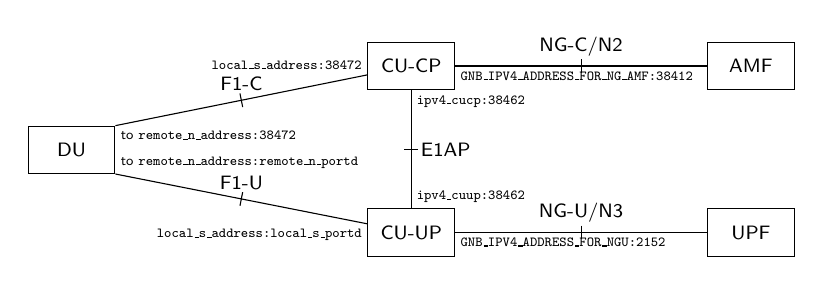
\begin{tikzpicture}
  [
    font=\scriptsize,
    node distance=1.5cm and 3.2cm,
    entity/.style={
      rectangle,
      draw,
      inner sep=0pt,
      minimum height=6mm,minimum width=11mm,
      align=center
    },
    split/.style={postaction={%
                      decorate,
                      decoration={
                          markings,mark={
                            at position \splitpos
                            with {
                              \draw (0pt,2.5pt) -- (0pt,-2.5pt);
                            }
                          }
                        }
                      }
                    },
    ip/.style={font=\tiny,outer sep=1pt,inner sep=1pt},
  ]
  \node[entity]                      (cu-cp) {CU-CP};
  \node[entity,below=of cu-cp]       (cu-up) {CU-UP};
  \node[entity,below left=0.45cm and 3.2cm of cu-cp]  (du)  {DU};
  \node[entity,right=of cu-cp] (amf) {AMF};
  \node[entity,right=of cu-up] (upf) {UPF};

  \draw[split,splitpos=0.5] (cu-cp) --
      node[ip,at start, below right, align=left] {\ip{GNB\_IPV4\_ADDRESS\_FOR\_NG\_AMF:38412}}
      node[above] {NG-C/N2}
      %node[ip,at end, below left] {127.0.1.10/24}
        (amf);
  \draw[split,splitpos=0.5] (cu-up) --
      node[ip, at start, below right,align=left] {\ip{GNB\_IPV4\_ADDRESS\_FOR\_NGU:2152}}
      node[above] {NG-U/N3}
      %node[ip, at end, below left] {127.0.1.10/24}
        (upf);
  \draw[split,splitpos=0.5] (cu-cp) --
      node[ip, at start, below right] {\ip{ipv4\_cucp:38462}}
      node[right] {E1AP}
      node[ip, at end, above right] {\ip{ipv4\_cuup:38462}}
        (cu-up);
  \draw[split] (du.north east)   --
      node[ip, at start, below right] {to \ip{remote\_n\_address:38472}}
      node[above] {F1-C}
      node[ip, at end, above left, align=right] {\ip{local\_s\_address:38472}}
        (cu-cp);
  \draw[split] (du.south east)   --
      node[ip, at start, above right] {to \ip{remote\_n\_address:remote\_n\_portd}}
      node[above] {F1-U}
      node[ip, at end, below left, align=right] {\ip{local\_s\_address:local\_s\_portd}}
        (cu-up);
\end{tikzpicture}
\end{document}
